\chapter{性能测试与优化分析}\label{chap:experiments}{
    \section{测试程序}


    \begin{enumerate}[leftmargin=1em, align=left]
        \item \textbf{WATER}:
              \begin{itemize}[leftmargin=*, nosep]
                  \item Water 是一个用于水分子动力学模拟的程序,它逐步模拟 n 个分子的运动状态。
                        其核心共享数据结构是一个一维数组,每个数组元素存储一个分子的多个特性参数,包括质心、受力、位移以及六个方向的导数等;
                  \item 在并行计算中,Water 采用均匀分配策略,将分子数组划分至各个处理机。
                        在每个时间步,每个处理机需计算本地分子与其他 n/2 个分子之间的相互作用力。
                        为减少通信开销,每个处理机维护一个本地备份以临时存储计算得到的作用力。
                        仅当所有处理机完成作用力计算后,才进入由锁保护的临界区,对全局结果进行更新。
                        不同时间步之间,处理机通过 barrier 操作实现同步;
              \end{itemize}
        \item \textbf{LU}:
              \begin{itemize}[leftmargin=*, nosep]
                  \item LU 采用块分解算法,将稠密矩阵分解为上三角矩阵和下三角矩阵,并使用连续块分配的 LU 分解策略。
                        连续块分配方法将原数组中非连续存储的矩阵块重新排列,使其在内存中连续存放,并分配至负责计算的处理机内存中,从而提高数据局部性和计算效率;
                  \item 块 LU 分解算法逐步进行,每次处理一列块。
                        每个步骤包括三个阶段:首先,对对角块进行 LU 分解;然后,将对角块下方的块除以已分解的对角块;
                        最后,更新矩阵右侧的剩余块(trailing blocks)。并行计算主要集中在第三阶段,而每个步骤的三个阶段通过 barrier 操作实现同步。;
              \end{itemize}
        \item \textbf{IS}:
              \begin{itemize}[leftmargin=*, nosep]
                  \item IS 是一个基于“桶排序”算法的整数排序程序。
                        它将 key 均匀分配到各个处理机,每个处理机维护一个私有“桶”,同时所有处理机共享一个公用“桶”;
                  \item 排序过程包括三个主要步骤:首先,每个处理机统计其私有“桶”中 key 的数量;
                        然后,在锁保护的临界区内,将这些计数累加到公用“桶”中;最后,根据公用“桶”中的信息构造出一个有序数组;
              \end{itemize}
        \item \textbf{SOR}:
              \begin{itemize}[leftmargin=*, nosep]
                  \item SOR 采用红黑格的逐次超松弛法(Successive Over-Relaxation, SOR)来求解偏微分方程。
                        在并行实现中,红黑两个数组被划分为大小接近的长方块,并分配给不同处理机进行计算;
                  \item 由于采用 5 点差分格式,仅在计算涉及带状区域边缘行时才需要通信。
                        每完成一次迭代后,各处理机通过 barrier 操作进行同步,确保所有处理机都能获取最新的计算结果;
              \end{itemize}
        \item \textbf{TSP}:
              \begin{itemize}[leftmargin=*, nosep]
                  \item TSP 采用分支限界算法求解旅行商问题,其核心数据结构包括:
                        用于存储路径的存储池、指向路径的优先队列、存放未使用路径指针的堆栈,以及记录当前最短路径的变量;
                  \item 在搜索最短路径的过程中,算法通过优先队列选择最有希望的路径进行扩展,并在必要时从存储池分配或释放路径。
                        随着搜索的进行,算法不断更新当前最短路径,并利用剪枝策略提高效率;
              \end{itemize}
        \item \textbf{EP}:
              \begin{itemize}[leftmargin=*, nosep]
                  \item EP 的主要目标是生成一组符合高斯分布的数对;
                  \item 该程序具有高度并行性,在整个计算过程中,唯一的通信操作仅发生在最后的累积阶段,用于合并各处理机的计算结果;
              \end{itemize}
        \item \textbf{PI}:
              \begin{itemize}[leftmargin=*, nosep]
                  \item PI 将pi的计算任务切分后分布到不同的主机上,分别计算后最后叠加;
                  \item 该程序具有高度并行性,最后通过对pi这个共享变量的操作将不同主机的计算结果累加;
              \end{itemize}
    \end{enumerate}

    \section{程序开销分析}
    本小节讨论的程序开销是指从主节点启动程序到所有节点完成任务并返回结果至主节点所耗费的总时间。
    在基于 M-JIAJIA 用户库的并行程序中,主要的开销包括系统初始化开销、计算开销和通信开销。
    下面对以上三种开销分别进行阐述:
    \begin{itemize}
        \item \textbf{系统初始化开销}:

              系统初始化开销代表调用 jia\_init() 初始化 M-JIAJIA 系统所耗费的时间。

              程序分发与远程执行产生的通信开销是系统初始化过程中最主要的性能瓶颈。
              当前,M-JIAJIA采用基于SCP(Secure Copy)的程序分发和SSH(Secure Shell)远程执行机制,
              其单线程串行传输模式导致分发时间随集群规模扩大呈线性增长(如图~\ref{fig:time-create-procs}所示),
              这种设计并不高效,未来可以通过并行分发策略和采用 RDMA 拷贝协议来降低该部分的开销。

              另一部分系统初始化开销是RDMA通信栈的初始化,这部分的开销如图~\ref{fig:time-init-rdma-comm}所示。
              目前已有研究~\citep{guo2024secm}尝试在建连阶段以流水线方式同时执行多个连接设置以降低该部分的开销。

        \item \textbf{计算开销}:

              计算开销指节点进行任务计算所需的时间。
              计算开销取决于任务规模、划分策略以及硬件性能等因素,但其对通信开销中的同步开销同样有重要影响。

              如图~\ref{fig:ep-performance}所示,基于 M-JIAJIA 的 ep 程序在多节点上执行,ep-i 中的 i 代表参与任务执行的节点数目,
              图中展示了 ep-8 所出现的反常现象,原因是参与并行任务的第八台节点(搭载 AMD EPYC 9754 128核处理器)处理速度过慢,
              导致其他节点在执行 barrier 同步时需要等待将近 17s 的时间(在节点 8 上单独执行 ep 程序需要近 159s 的时间,
              是其他节点单独执行的6-7倍)。因此,合理的计算集群构建方案是采用处理速度相近的节点,或根据处理能力划分任务。

        \item \textbf{通信开销}

              通信开销可以分为两部分,一是因访问远程数据导致的开销,二是维护一致性导致的开销。
              这部分将在 5.3 小节进一步介绍。

    \end{itemize}

    \begin{figure}
        \centering
        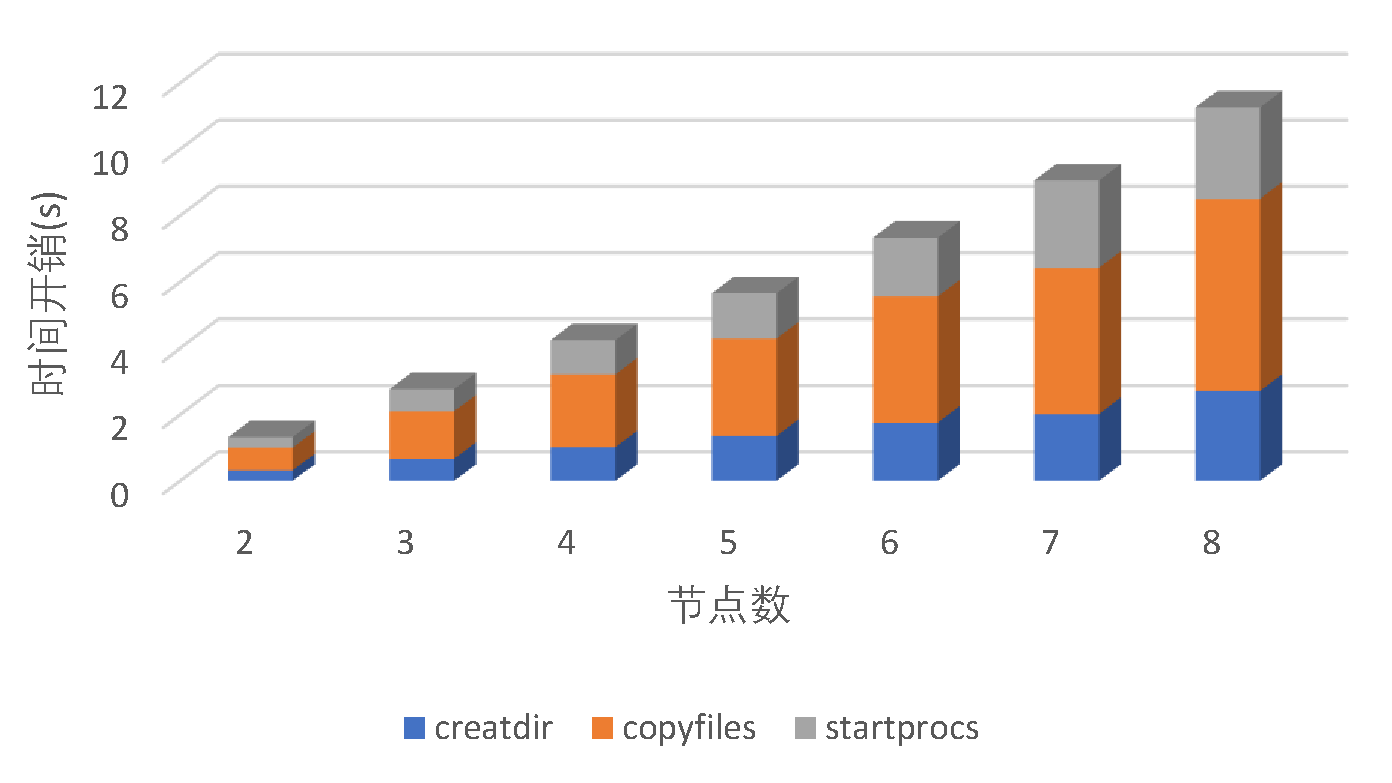
\includegraphics[width=0.85\linewidth]{Img/程序不同集群规模开销.pdf}
        \bicaption{\enspace 程序分发执行在不同集群规模下的开销}{\enspace Cost of Program Distribution and Launch with Varying Cluster Sizes}
        \label{fig:time-create-procs}
        {\footnotesize \par 注:测试在千兆以太网环境下进行,网络接口速度 1000 Mbps,采用 UDP 通信协议}
    \end{figure}

    \begin{figure}[!htbp]
        \centering
        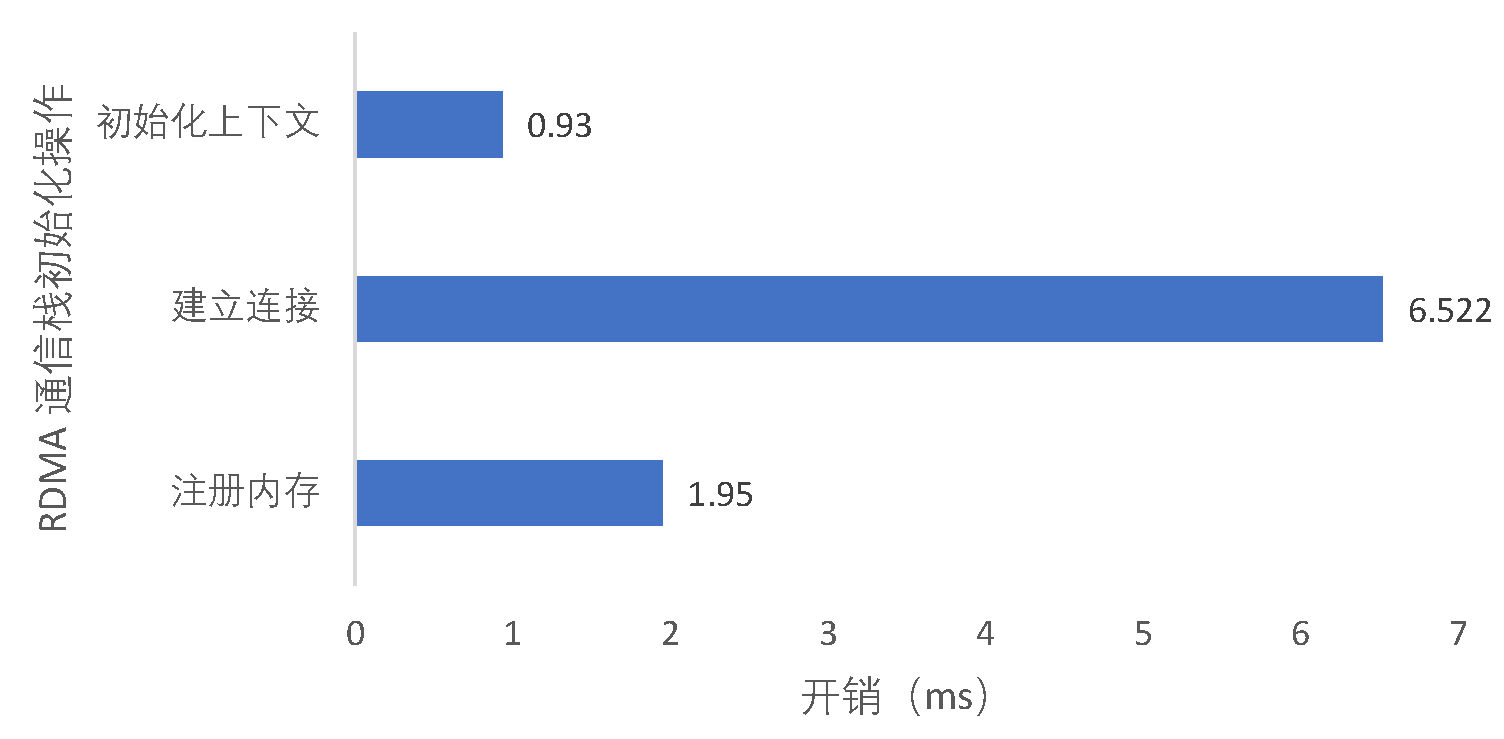
\includegraphics[width=0.85\linewidth]{Img/RDMA通信栈初始化开销分析.pdf}
        \bicaption{\enspace RDMA通信栈初始化开销分析}{\enspace RDMA Communication Stack Initialization Cost Analysis}
        \label{fig:time-init-rdma-comm}
        {\footnotesize \par 注:测试在两台配备 Mellanox ConnectX-3 Pro 网卡的工作站之间进行}
    \end{figure}

    \begin{figure}[!htbp]
        \centering
        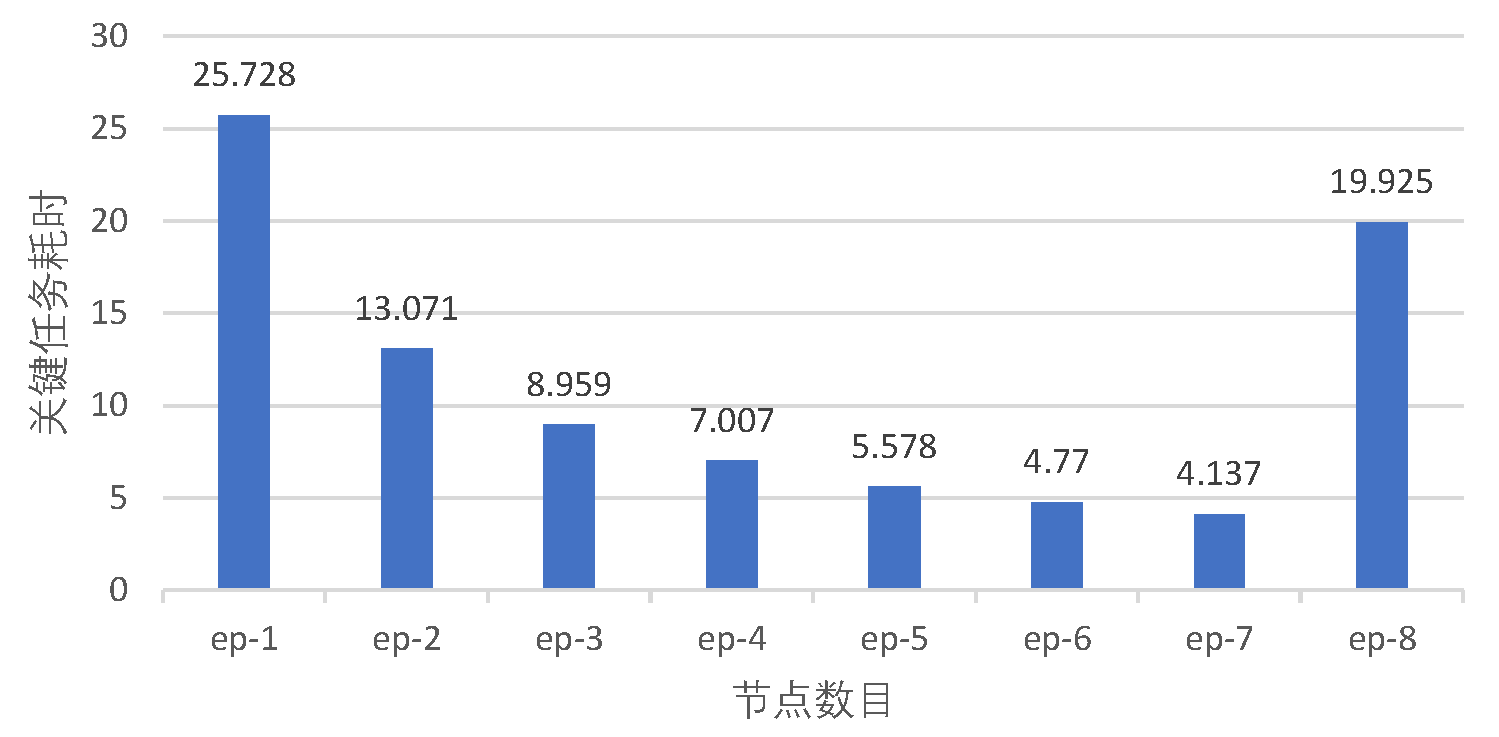
\includegraphics[width=\linewidth]{Img/EP-performance.pdf}
        \bicaption{\enspace 并行程序 ep 在不同节点数下的性能表现}{\enspace Parallel Program EP Performance on Varying Node Counts}
        \label{fig:ep-performance}
        {\footnotesize \par 注:测试在千兆以太网环境下进行,采用 UDP通信,
            测试节点1/2/3 搭载 Intel Xeon Gold 6338 CPU @ 2.000GHz 处理器,
            节点4/5/6搭载 Intel Xeon Platinum 8176 CPU @ 2.10GHz 处理器,
            节点 7 搭载AMD EPYC 9654 96-Core 处理器,
            节点 8 搭载AMD EPYC 9654 128-Core 处理器}
    \end{figure}

    \section{RDMA 通信栈 VS UDP 通信栈}

    M-JIAJIA 系统的 UDP 和 RDMA 通信栈对比测试在两台戴尔 Precision 3660 塔式工作站之间进行。
    每台工作站配备 16 核第 12 代英特尔Core i9-12900K 处理器和 62.5GB 内存;UDP 通信栈通过千兆以太网进行数据传输,
    而 RDMA 通信栈依托 Mellanox ConnectX-3 Pro 网卡(最大带宽达 56000Mb/s),在 InfiniBand 模式下实现 RDMA 通信;
    测试程序依次是 water(288个分子)、lu($1024\times1024$)、ep($2^{28}$)、is($2^{22}$)、mm($1024\times1024$)、
    pi($10^6$个区间)、tsp(19个城市)、sor($256\times2048$)。

    图~\ref{fig:time-comparison-diff-stacks}显示了测试程序集在UDP、IPoIB与RDMA通信协议栈下执行的性能,
    横轴为各个测试程序,纵轴为主节点上程序运行时间,包含系统初始化开销。

    \begin{figure}[!htbp]
        \centering
        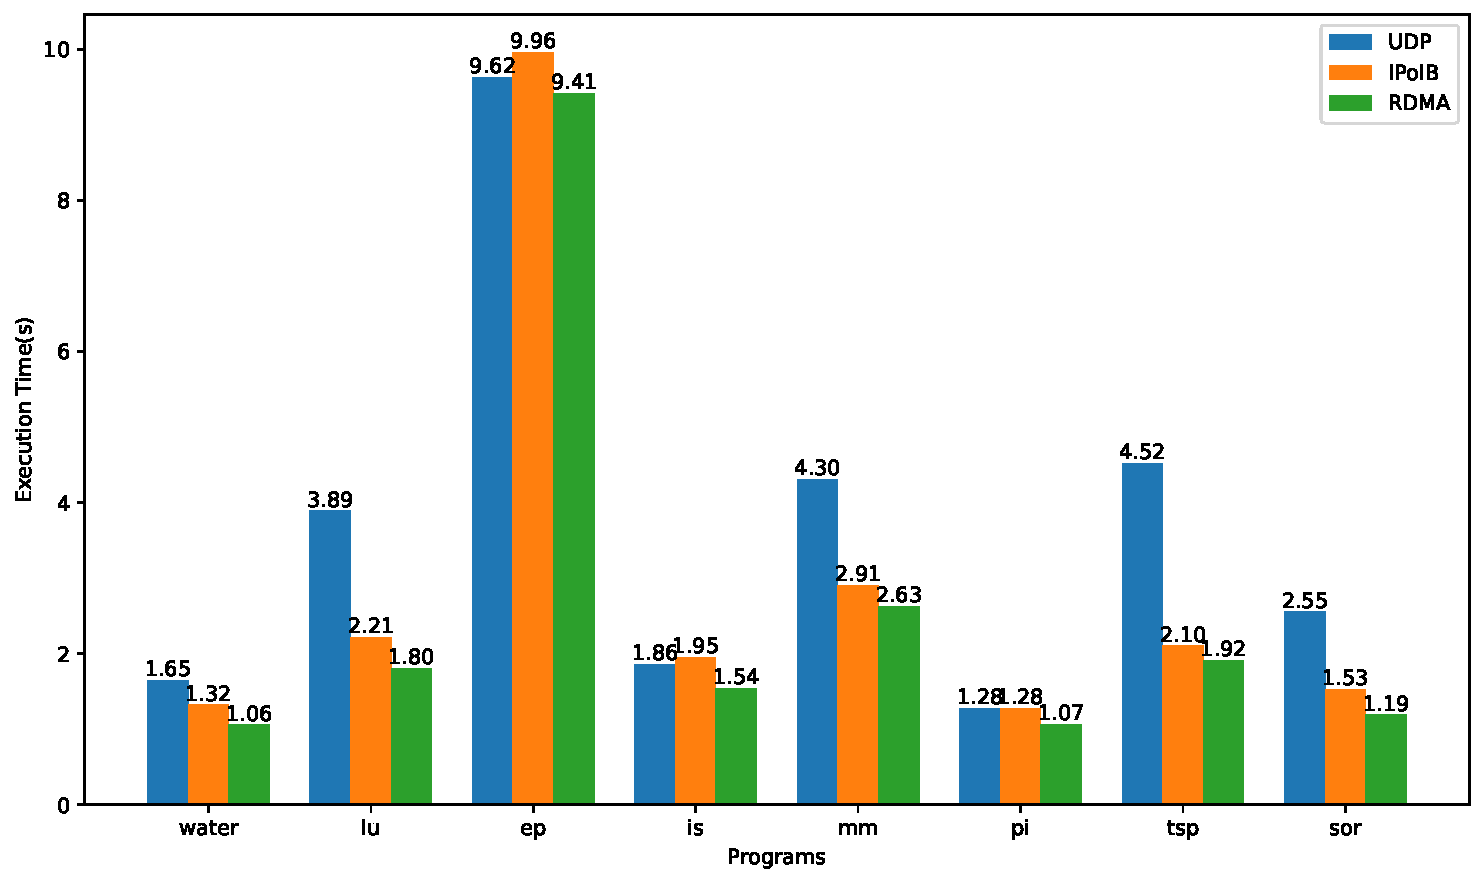
\includegraphics[width=\linewidth]{Img/execution_time_comparison.pdf}
        \bicaption{\enspace 不同通信栈下程序执行时间比较}{\enspace Comparison of Program Execution Time Across Different Communication Stacks}
        \label{fig:time-comparison-diff-stacks}
    \end{figure}

    结果表明,与 UDP 和 IPoIB 通信栈相比,RDMA 通信栈总是可以取得更优的性能。
    具体而言,相比于 UDP 通信栈下运行的程序,RDMA 通信栈下运行的程序性能分别提升了 water(35.94\%)、lu(53.71\%)、
    ep(2.16\%)、is(16.86\%)、mm(38.84\%)、pi(16.56\%)、tsp(57.52\%)与sor(53.39\%);
    相比于IPoIB,程序性能提升了  water(20.06\%)、lu(18.64\%)、
    ep(5.48\%)、is(21.00\%)、mm(9.49\%)、pi(16.48\%)、tsp(8.57\%)与sor(22.12\%)。
    这些程序性能提升差异的主要原因是程序的系统初始化开销、计算开销与通信开销占总开销的比例不同。

    部分程序性能的提升主要得益于同步开销的降低,这类程序通常不执行远程取页操作或仅在非主节点上执行远程取页操作,
    测试程序中的 water、ep、is与pi属于此类(如表~\ref{tab:type1-time}所示)。
    同步开销包括 barrier 和 lock 原语的执行时间,而其具体开销来源于请求同步变量(如锁或屏障)的成本以及传播 diffs 的开销。

    部分程序的性能提升主要体现在远程取页开销的降低上。
    这些程序包括 lu、mm 与 sor (详见表~\ref{tab:type2-time})。
    通过比较不同通信栈下相同数量远程取页的耗时差异,可以看出RDMA通信栈相较于UDP通信栈快了约18倍,相较于IPoIB快了2-3倍。
    同时,实验数据显示,本地访问一页触发段违例处理需要 4-5us,而在RDMA通信栈下远程访问一页触发段违例处理需要60-90us,这表明两者之间仍有一个数量级的差距。

    \begin{table}
        \footnotesize% fontsize
        \setlength{\tabcolsep}{4pt}% column separation
        \renewcommand{\arraystretch}{1.5}% row space 
        \centering
        \bicaption{不同通信栈下主节点部分程序的同步开销}{Synchronization Costs of Master Node Programs on Different Communication Stack}% caption
        \label{tab:type1-time}
        \begin{tabular}{l|c|c|c}
            \hline
            %\multicolumn{num_of_cols_to_merge}{alignment}{contents} \\
            %\cline{i-j}% partial hline from column i to column j
                        & Barrier 执行时间(个数) & Lock 执行时间(个数) & 同步时间(ms) \\
            \hline
            water-UDP   & 630.60 (35)      & 37.88 (35)    & 667.48   \\
            water-IPoIB & 322.26           & 4.85          & 327.11   \\
            water-RDMA  & 22.44            & 3.27          & 25.71    \\
            \hline
            ep-UDP      & 284.61 (3)       & 0.44 (1)      & 285.05   \\
            ep-IPoIB    & 285.60           & 0.44          & 286.04   \\
            ep-RDMA     & 4.23             & 0.30          & 4.53     \\
            \hline
            is-UDP      & 371.69 (32)      & 8.38 (10)     & 380.07   \\
            is-IPoIB    & 314.98           & 1.99          & 316.97   \\
            is-RDMA     & 8.65             & 0.94          & 9.59     \\
            \hline
            pi-UDP      & 289.88 (3)       & 5.88 (1)      & 295.76   \\
            pi-IPoIB    & 269.24           & 2.42          & 271.66   \\
            pi-RDMA     & 7.37             & 0.33          & 7.7      \\
            \hline
            tsp-UDP     & 3.31 (2)         & 2614.50 (380) & 2617.81  \\
            tsp-IPoIB   & 2.27             & 169.07        & 171.34   \\
            tsp-RDMA    & 0.84             & 43.82         & 44.66    \\
            \hline
        \end{tabular}
    \end{table}

    \begin{table}[!htbp]
        \footnotesize% fontsize
        \setlength{\tabcolsep}{4pt}% column separation
        \renewcommand{\arraystretch}{1.5}% row space 
        \centering
        \bicaption{不同通信栈下主节点部分程序的开销}{Costs of Master Node Programs on Different Communication Stack}% caption
        \label{tab:type2-time}
        \begin{tabular}{l|c|c|c|c}
            \hline
            %\multicolumn{num_of_cols_to_merge}{alignment}{contents} \\
            %\cline{i-j}% partial hline from column i to column j
                      & Barrier执行时间(个数) & 远程取页时间(页数)     & 通信总开销(ms) & 本地取页时间(页数)  \\
            \hline
            lu-UDP    & 938.25 (68)     & 818.11 (689)   & 1756.36   & 12.87(2770) \\
            lu-IPoIB  & 145.65          & 135.9          & 281.55    & 13.04       \\
            lu-RDMA   & 52.09           & 44.71          & 96.8      & 13.46       \\
            \hline
            mm-UDP    & 529.12 (3)      & 1277.84 (1024) & 1806.96   & 6.55(1536)  \\
            mm-IPoIB  & 319.11          & 144.5          & 463.61    & 7.02        \\
            mm-RDMA   & 19.74           & 69.31          & 89.05     & 6.29        \\
            \hline
            sor-UDP   & 496.48 (201)    & 325.31 (199)   & 821.79    & 1.38(324)   \\
            sor-IPoIB & 46.95           & 43.42          & 90.37     & 1.58        \\
            sor-RDMA  & 22.33           & 19.06          & 41.39     & 2.26        \\
            \hline
        \end{tabular}
    \end{table}




    \section{远程预取优化效果分析}
    \begin{figure}[!htbp]
        \centering
        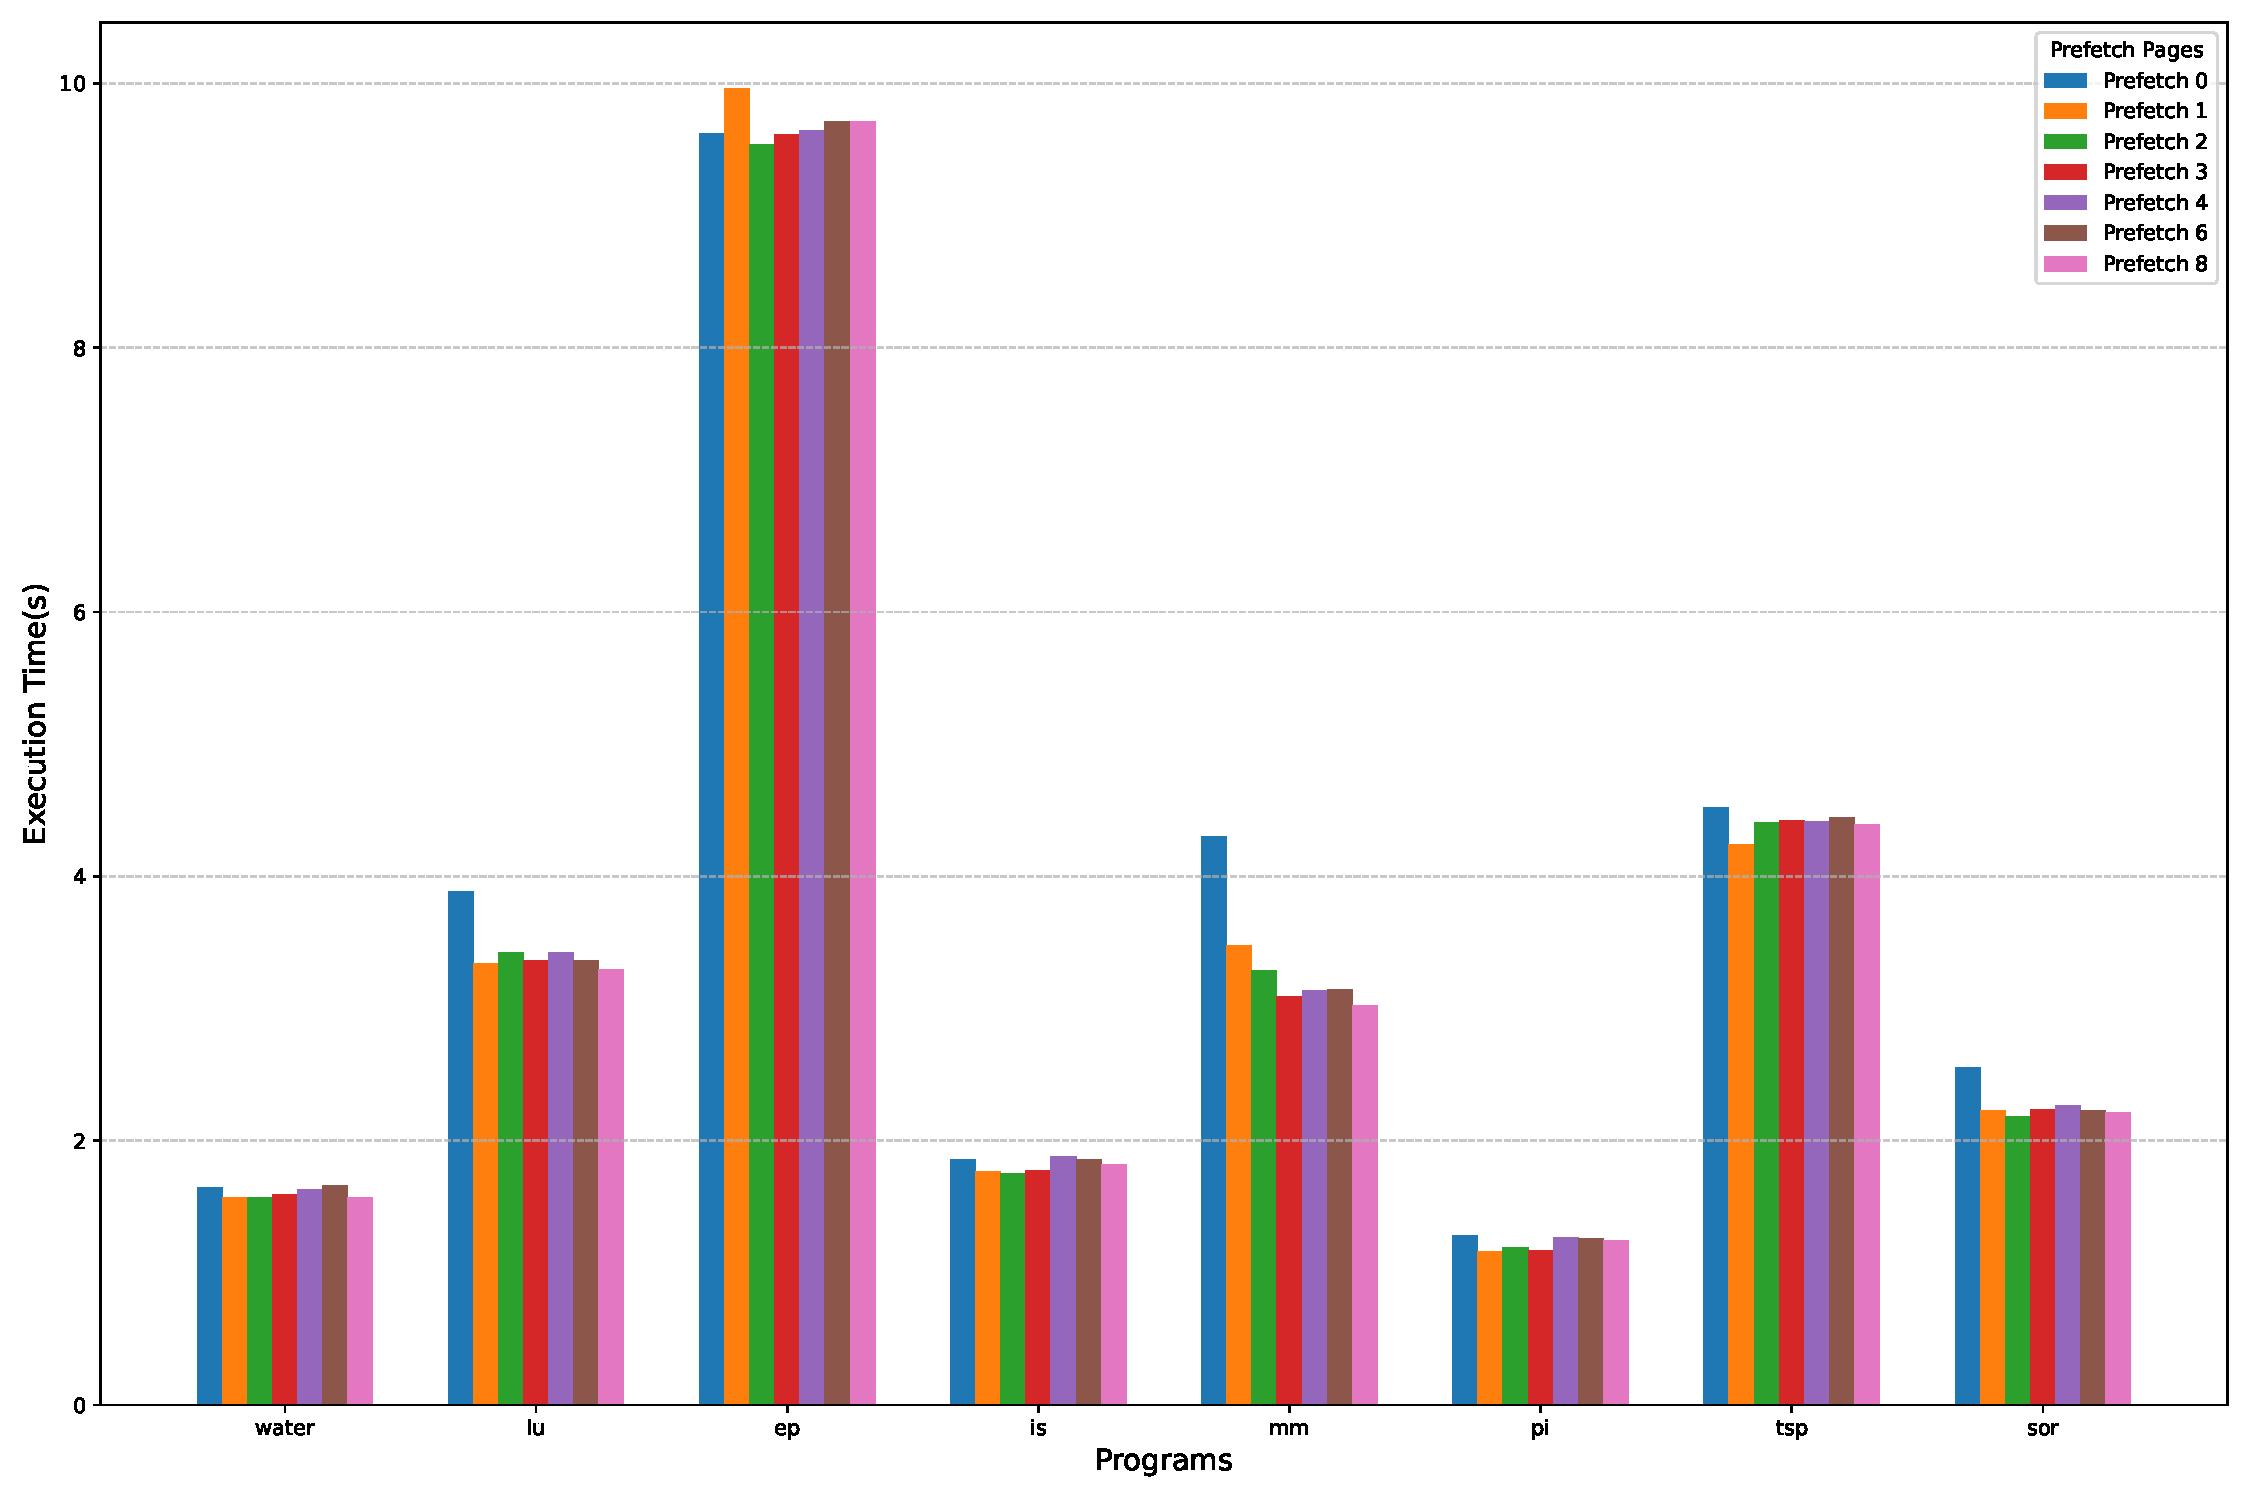
\includegraphics[width=0.90\linewidth]{Img/udp_prefetch_execution_time.pdf}
        \bicaption{UDP通信栈:程序性能与预取页数关系图}{UDP/IP Stack: Program Performance vs Prefetch Pages Relationship Diagram}
        \label{fig:udp-prefetch-result}
    \end{figure}
    图 ~\ref{fig:udp-prefetch-result} 展示了在 UDP 通信栈环境下,不同程序在不同预取页数条件下的执行性能表现。
    测试采用的环境与第 5.3 小节中详述的 UDP 通信栈测试环境保持一致。
    实验结果表明,预取优化策略对多数程序的性能产生了显著影响。其中,lu、mm 和 sor 程序的性能提升尤为突出,分别实现了 13\%、41\% 和 12\% 的性能优化。
    分析原因是这些程序在运行过程中分配了较大规模的共享内存,预取机制发挥了关键作用,有效提升了整体性能。

    \begin{figure}
        \centering
        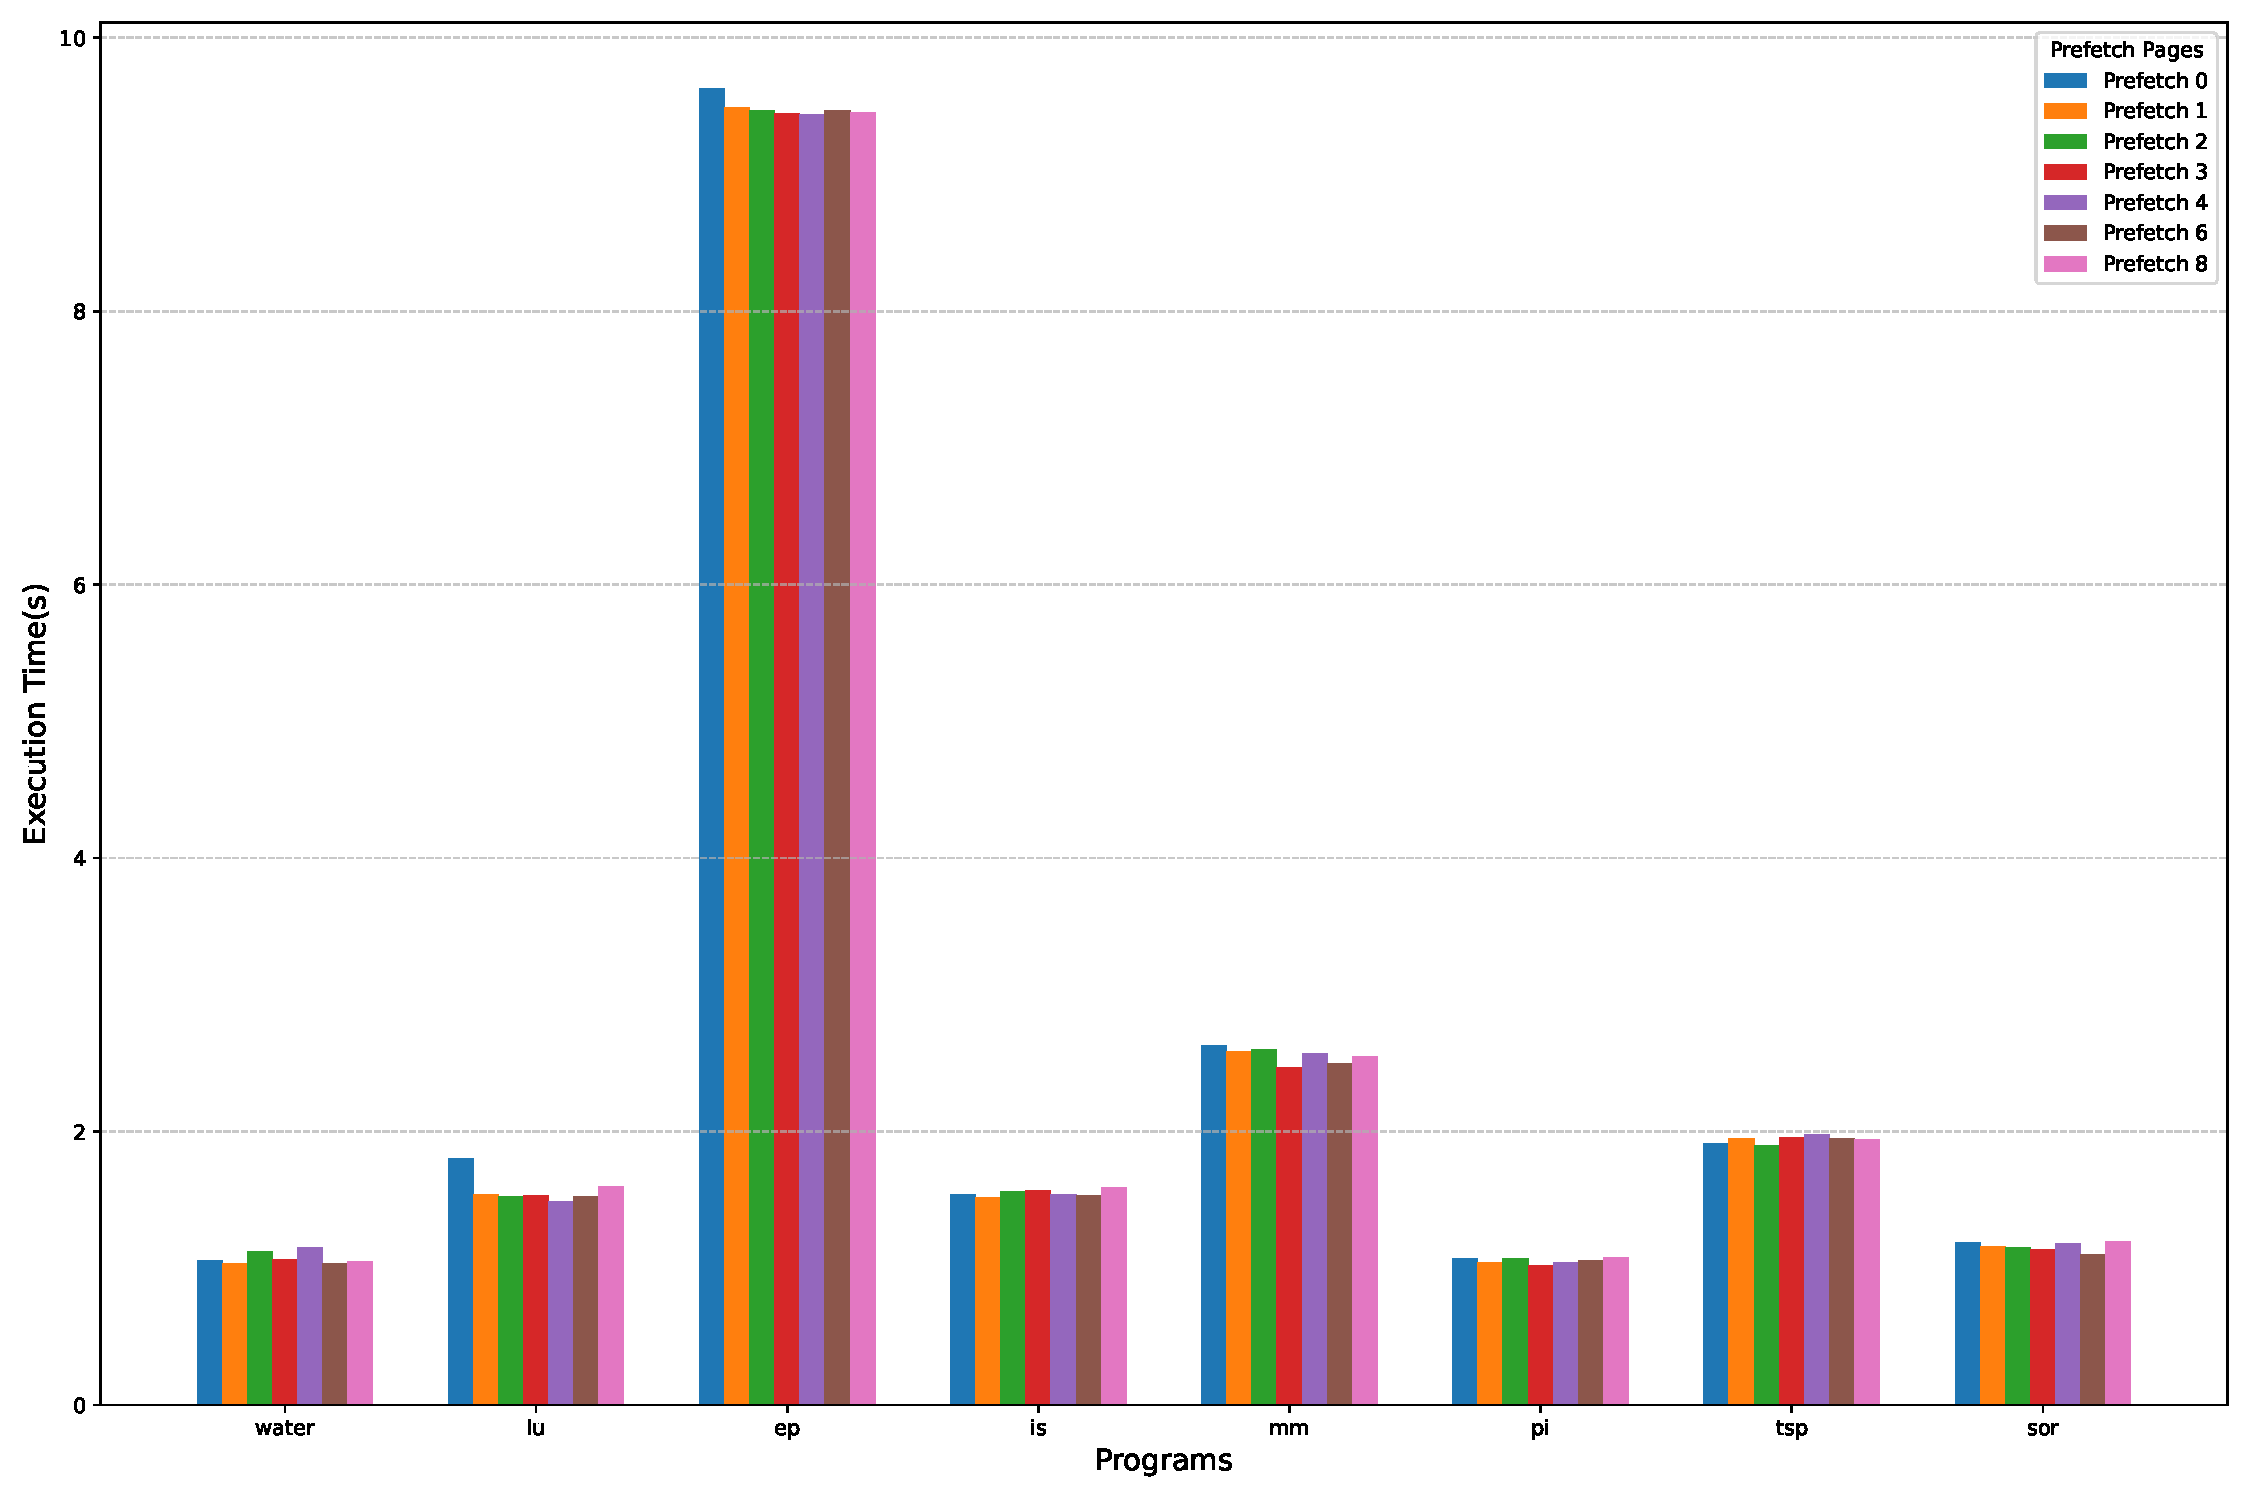
\includegraphics[width=0.90\linewidth]{Img/rdma_prefetch_execution_time.pdf}
        \bicaption{RDMA通信栈:程序性能与预取页数关系图}{RDMA Stack: Program Performance vs Prefetch Pages Relationship Diagram}
        \label{fig:rdma-prefetch-result}
    \end{figure}

    图~\ref{fig:rdma-prefetch-result} 展示了在 RDMA 通信栈环境下,不同程序在不同预取页数条件下的执行性能表现。
    测试采用的环境与第 5.3 小节中详述的 RDMA 通信栈测试环境保持一致。
    实验结果表明,除了 lu 程序依旧可以获得较为明显的性能提升外,其余程序由于通信延迟的显著降低,预取优化的效果并不明显。
    分析原因是RDMA网络技术本身的传输性能已经很好,因此再进行预取优化对性能的影响并不显著。

    \section{类 MPI 接口测试}
    M-JIAJIA 提供了类似于消息传递的基础通信接口 jia\_send 和 jia\_recv。
    图~\ref{fig:test-mpi} 展示了在不同通信栈下,这两个接口传输不同数据量时的性能表现,并与 OpenMPI 的 MPI\_send 和 MPI\_recv 在单机双进程间的性能进行了对比。
    测试环境与第 5.3 小节中详细描述的 RDMA 通信栈测试环境保持一致,OpenMPI 的测试版本为 5.0.6。实验结果如下:

    \begin{figure}[!htbp]
        \centering
        \begin{subfigure}[b]{0.8\textwidth}
            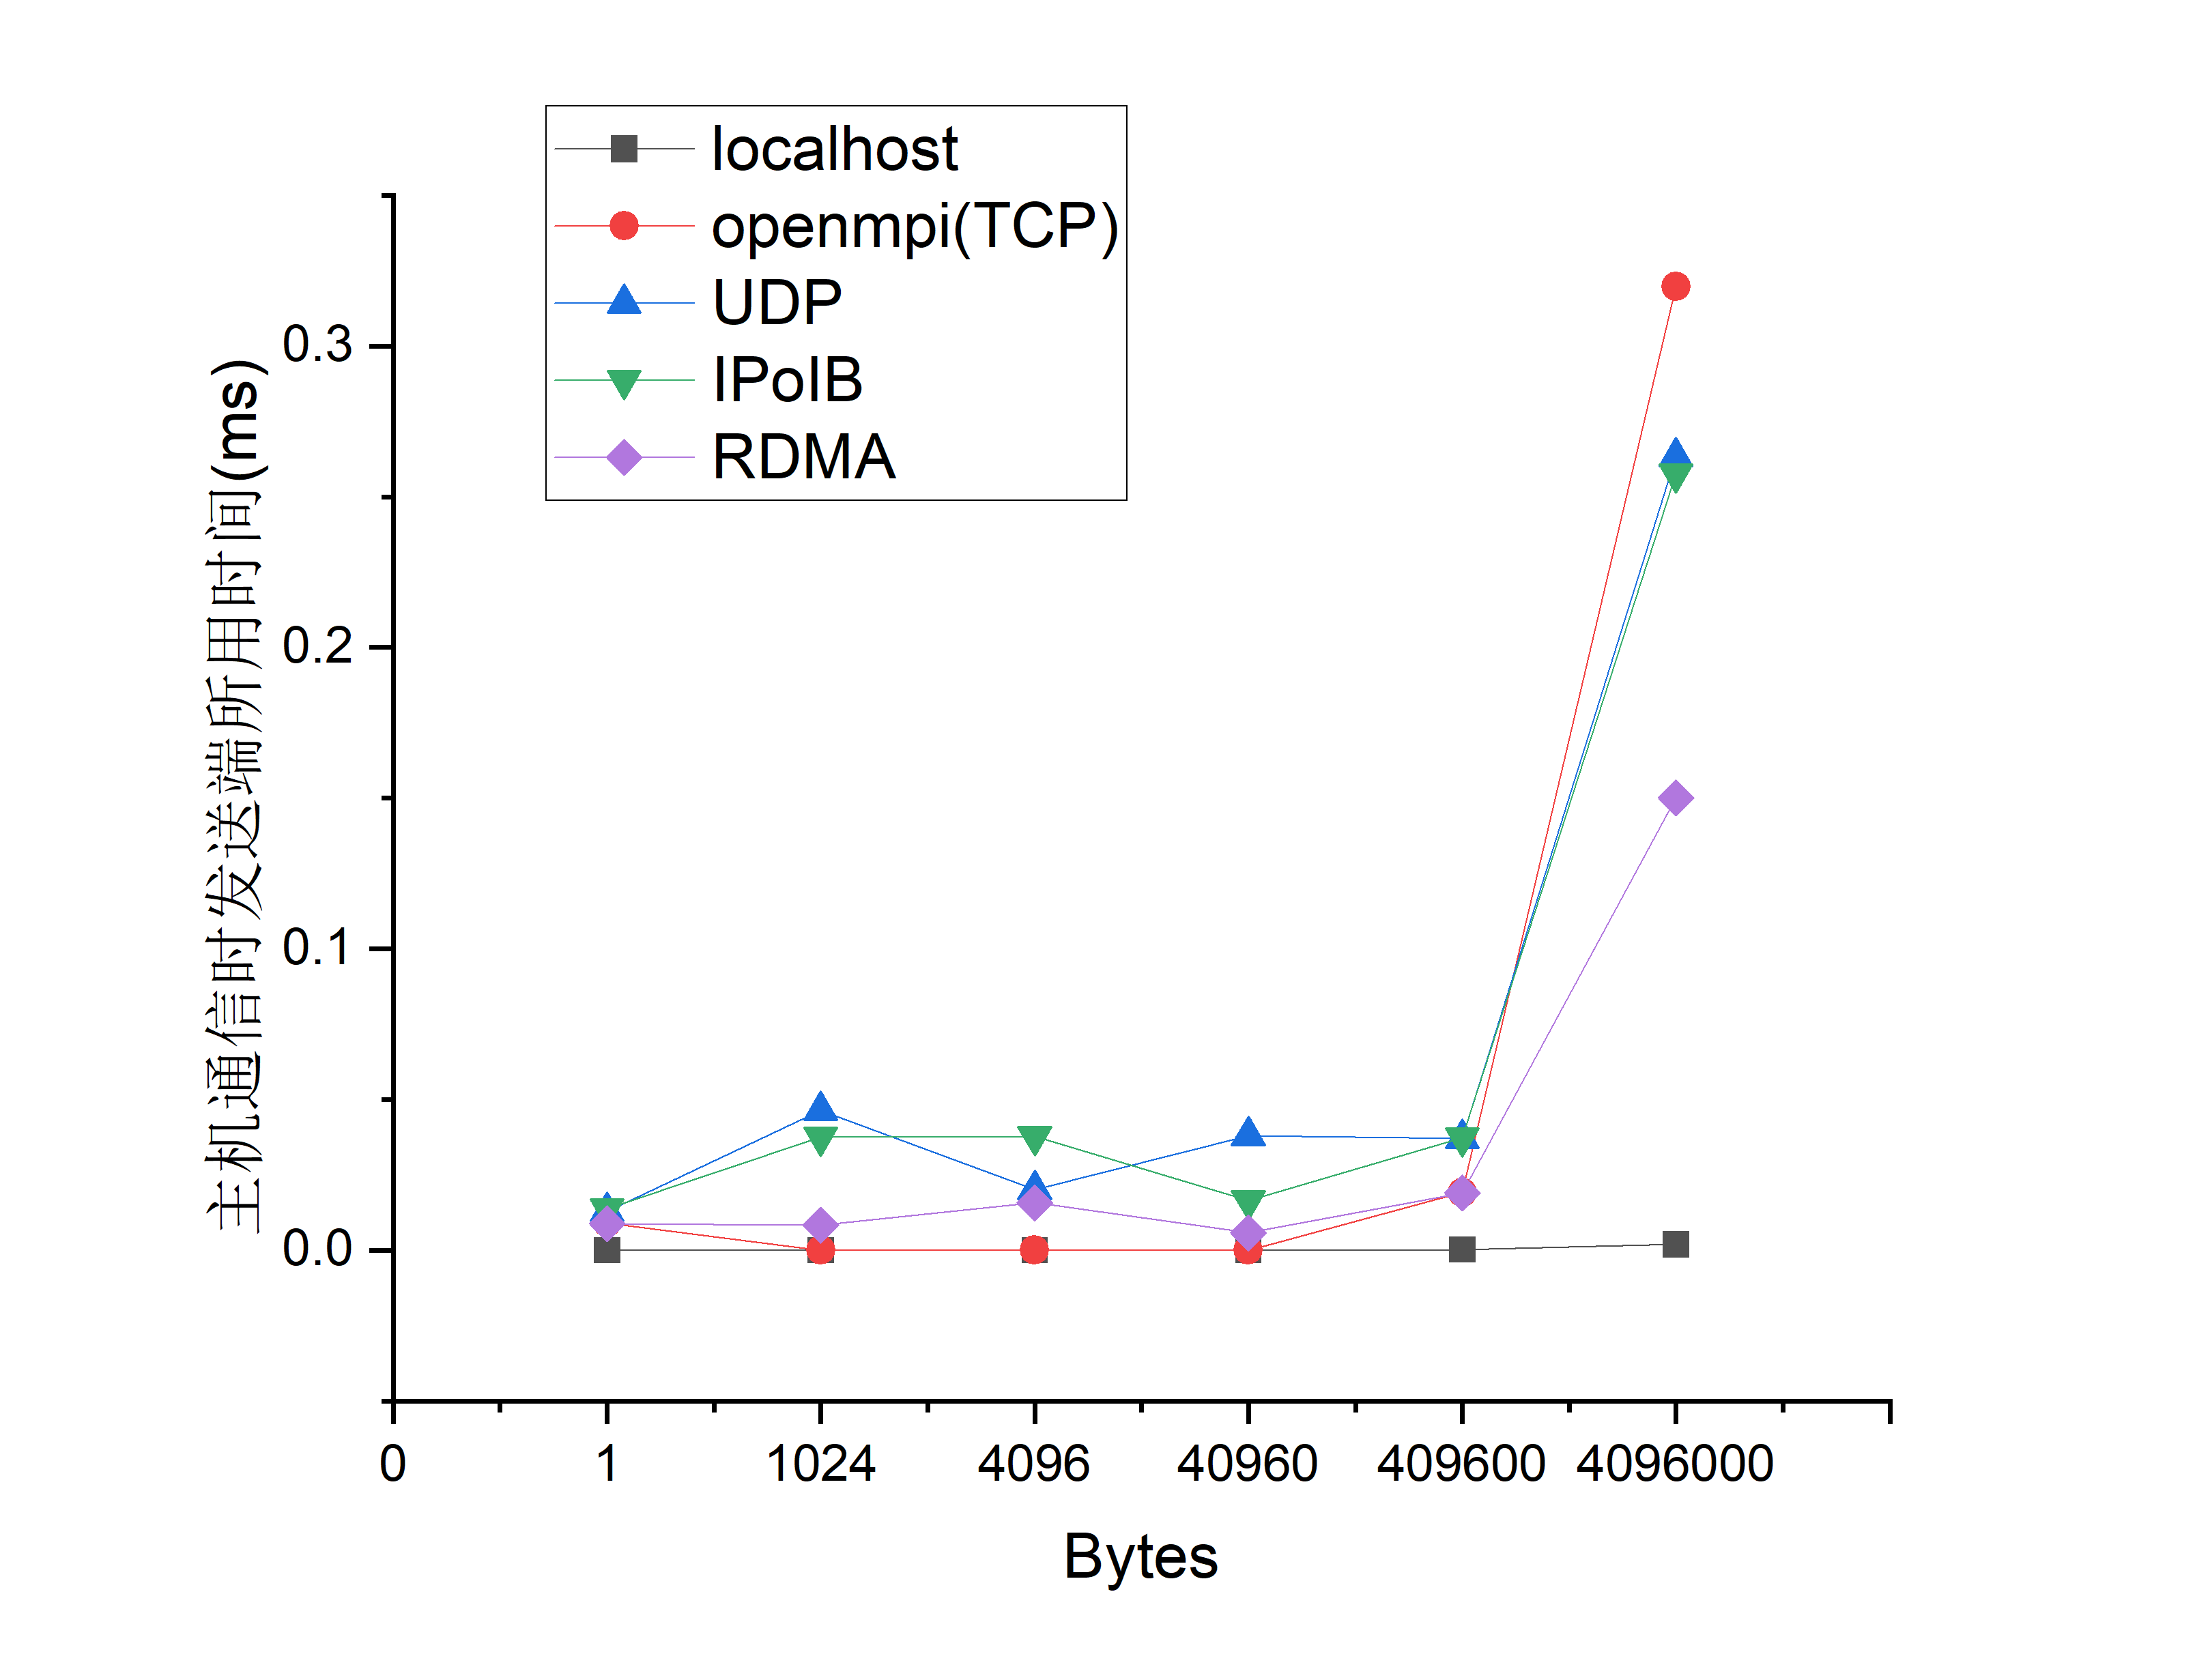
\includegraphics[width=1.0\textwidth]{Img/send_perf.png}
            \caption{jia\_send 接口性能测试}
            \label{fig:test-send}
        \end{subfigure}
        ~ % 添加期望的间隔
        \begin{subfigure}[b]{0.8\textwidth}
            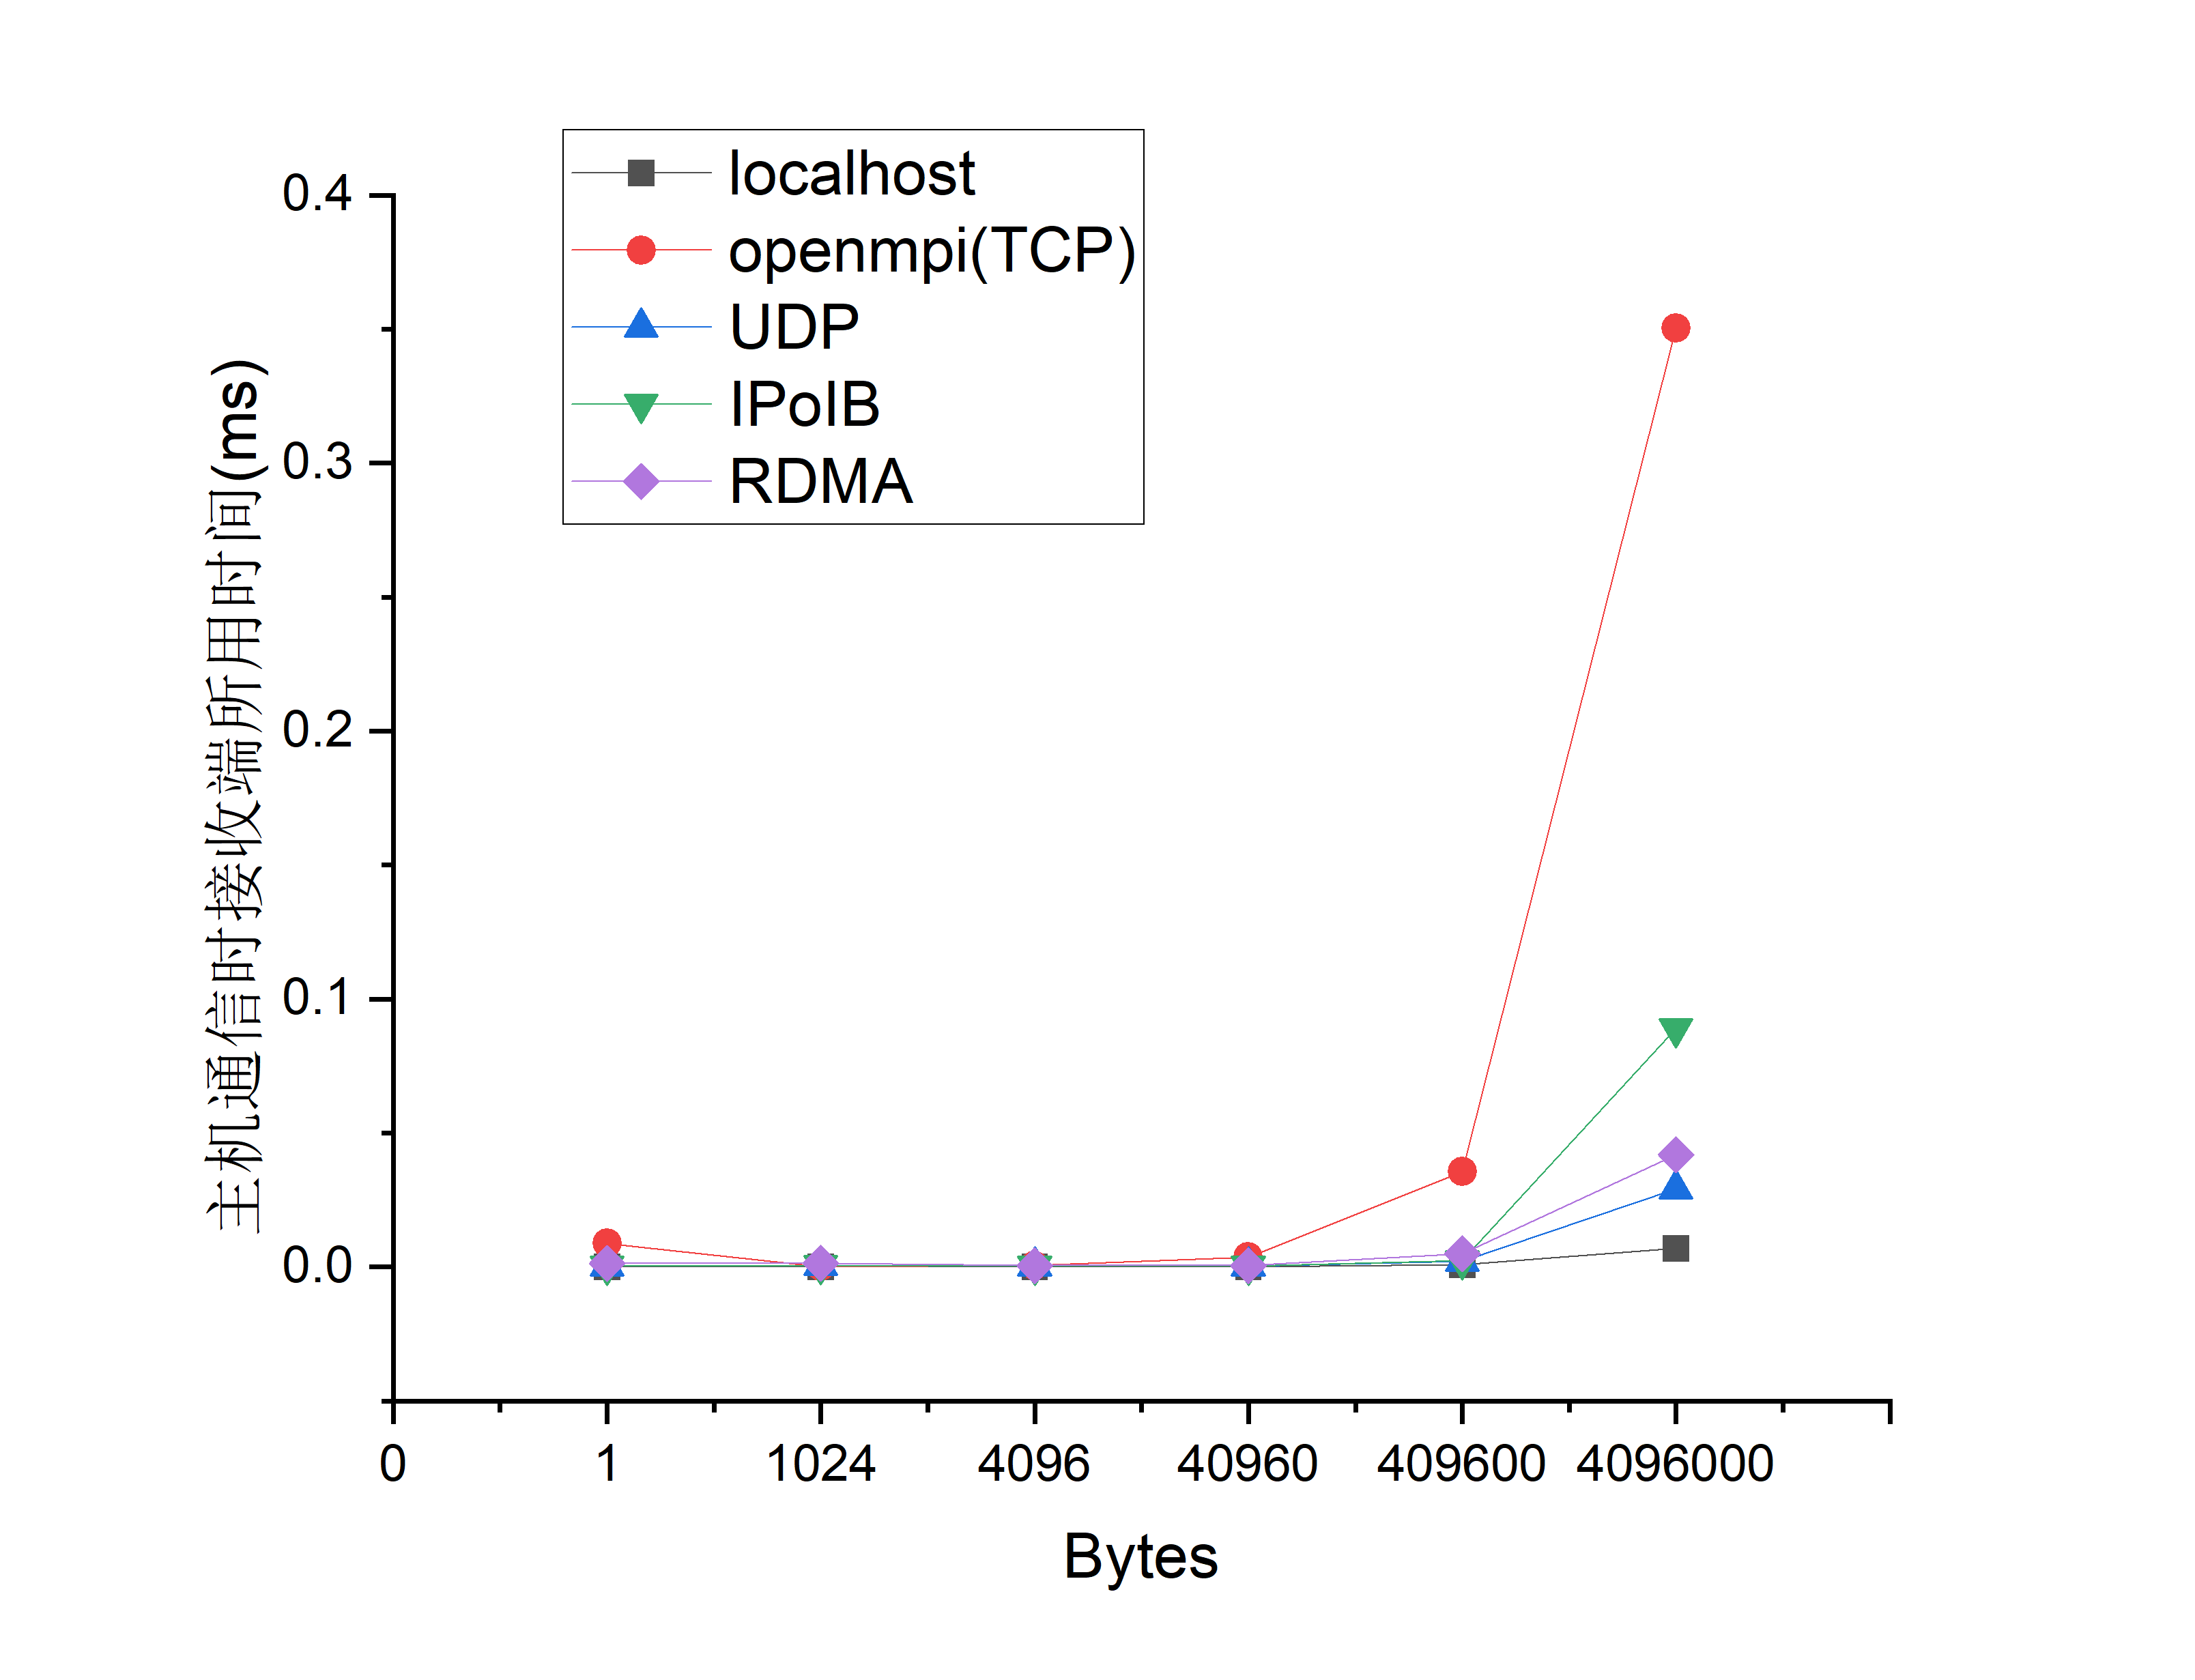
\includegraphics[width=1.0\textwidth]{Img/recv_perf.png}
            \caption{jia\_recv 接口性能测试}
            \label{fig:test-recv}
        \end{subfigure}
        \bicaption{\enspace 消息传递接口性能比较}{\enspace Performance Comparison of Message Passing Interfaces}
        \label{fig:test-mpi}
    \end{figure}

    由以上实验数据统计图可以看出:
    \begin{itemize}
        \item 接收端四种通信方式在小于40960字节时花费时间大致一致,大于40960字节时TCP连接花费时间显著多于另外三种连接花费时间;
              同时UDP,IPoIB与RDMA三种连接方式花费时间大致一致,没有显著区别;
        \item 发送端四种通信方式在小于409600字节时花费时间没有显著区别,波动属于正常区间;
              大于409600字节时TCP,UDP与IPoIB花费时间显著增长,明显多于RDMA发送端花费的时间(约为RDMA花费时间的2倍);
        \item 综合接收端与发送端所花费的时间可以看出,在大文件网络传输的情况下,TCP连接接收端与发送端花费时间均为最长(总时间最长);
              UDP与IPoIB网络连接总体花费时间大致一致,IpoIB在接收端花费的时间略长一些;RDMA连接花费的时间最短,且在发送端显著低于其他四种连接方式。
    \end{itemize}

    \section{本章小结}
    本章 5.1 小节具体介绍 Water、LU、EP、IS、MM、PI、TSP和SOR 八个测试程序。

    本章 5.2 小节将基于 M-JIAJIA 的程序开销细分为系统初始化开销、计算开销和通信开销三个部分,
    并探讨了系统初始化开销和计算开销的主要构成。

    本章 5.3 小节主要比较了 UDP、IPoIB 和 RDMA 三种通信栈下测试程序的执行时间,
    并重点比较了RDMA相较UDP通信栈在性能上的提升,分析了性能提升与开销降低的关系。

    本章 5.4 小节探讨了远程预取在 UDP 和 RDMA 通信栈中的优化效果。

    本章 5.5 小节主要对比 UDP、IPoIB 和 RDMA 三种通信栈下M-JIAJIA类消息传递接口的性能,
    并与OpenMPI 单机多进程之间的消息传递性能进行了比较,重点比较了大字节传输时的性能提升。
}